% chktex-file 8
% chktex-file 13

\documentclass{article}
\usepackage{amsmath}
\usepackage{hyperref}
\usepackage{xcolor}
\usepackage{ulem}
\usepackage{graphicx}
\usepackage[margin=0.75in]{geometry}

\graphicspath{ {./images/} }

\definecolor{darkblue}{rgb}{0, 0, 20}

\hypersetup{
    colorlinks=true,
    urlcolor=darkblue,
    linkcolor=blue,
    filecolor=magenta,
    citecolor=blue,
}

\title{EgoCVR: An Egocentric Benchmark for Fine-Grained Composed Video Retrieval}
\author{Thomas Hummel, Shyamgopal Karthik, Mariana-Iuliana Georgescu, Zeynep Akata}
\date{}
\setlength{\parindent}{0pt}

\begin{document}

\maketitle

\begin{center}\textbf{Accepted for ECCV 2024 (\href{https://arxiv.org/pdf/2407.16658}{Paper}) (\href{https://github.com/ExplainableML/EgoCVR}{GitHub})}\end{center}

The paper introduces EgoCVR, an evaluation benchmark for fine-grained CVR that focuses on temporal video understanding rather than object modifications. The authors also introduce a training-free method that combines LLM-based text refinement and visual filtering for composed video retrieval.

\section*{Motivation}

85\% of WebVid-CoVR-Test samples involve object-centered modifications, such as color or shape changes, which can be solved with image-based methods and do not require temporal understanding. Also, videos in the WebVid-CoVR-Test dataset were paired through single-word differences in video captions, which does not properly test models on diverse and complex modifications.

\begin{center}
    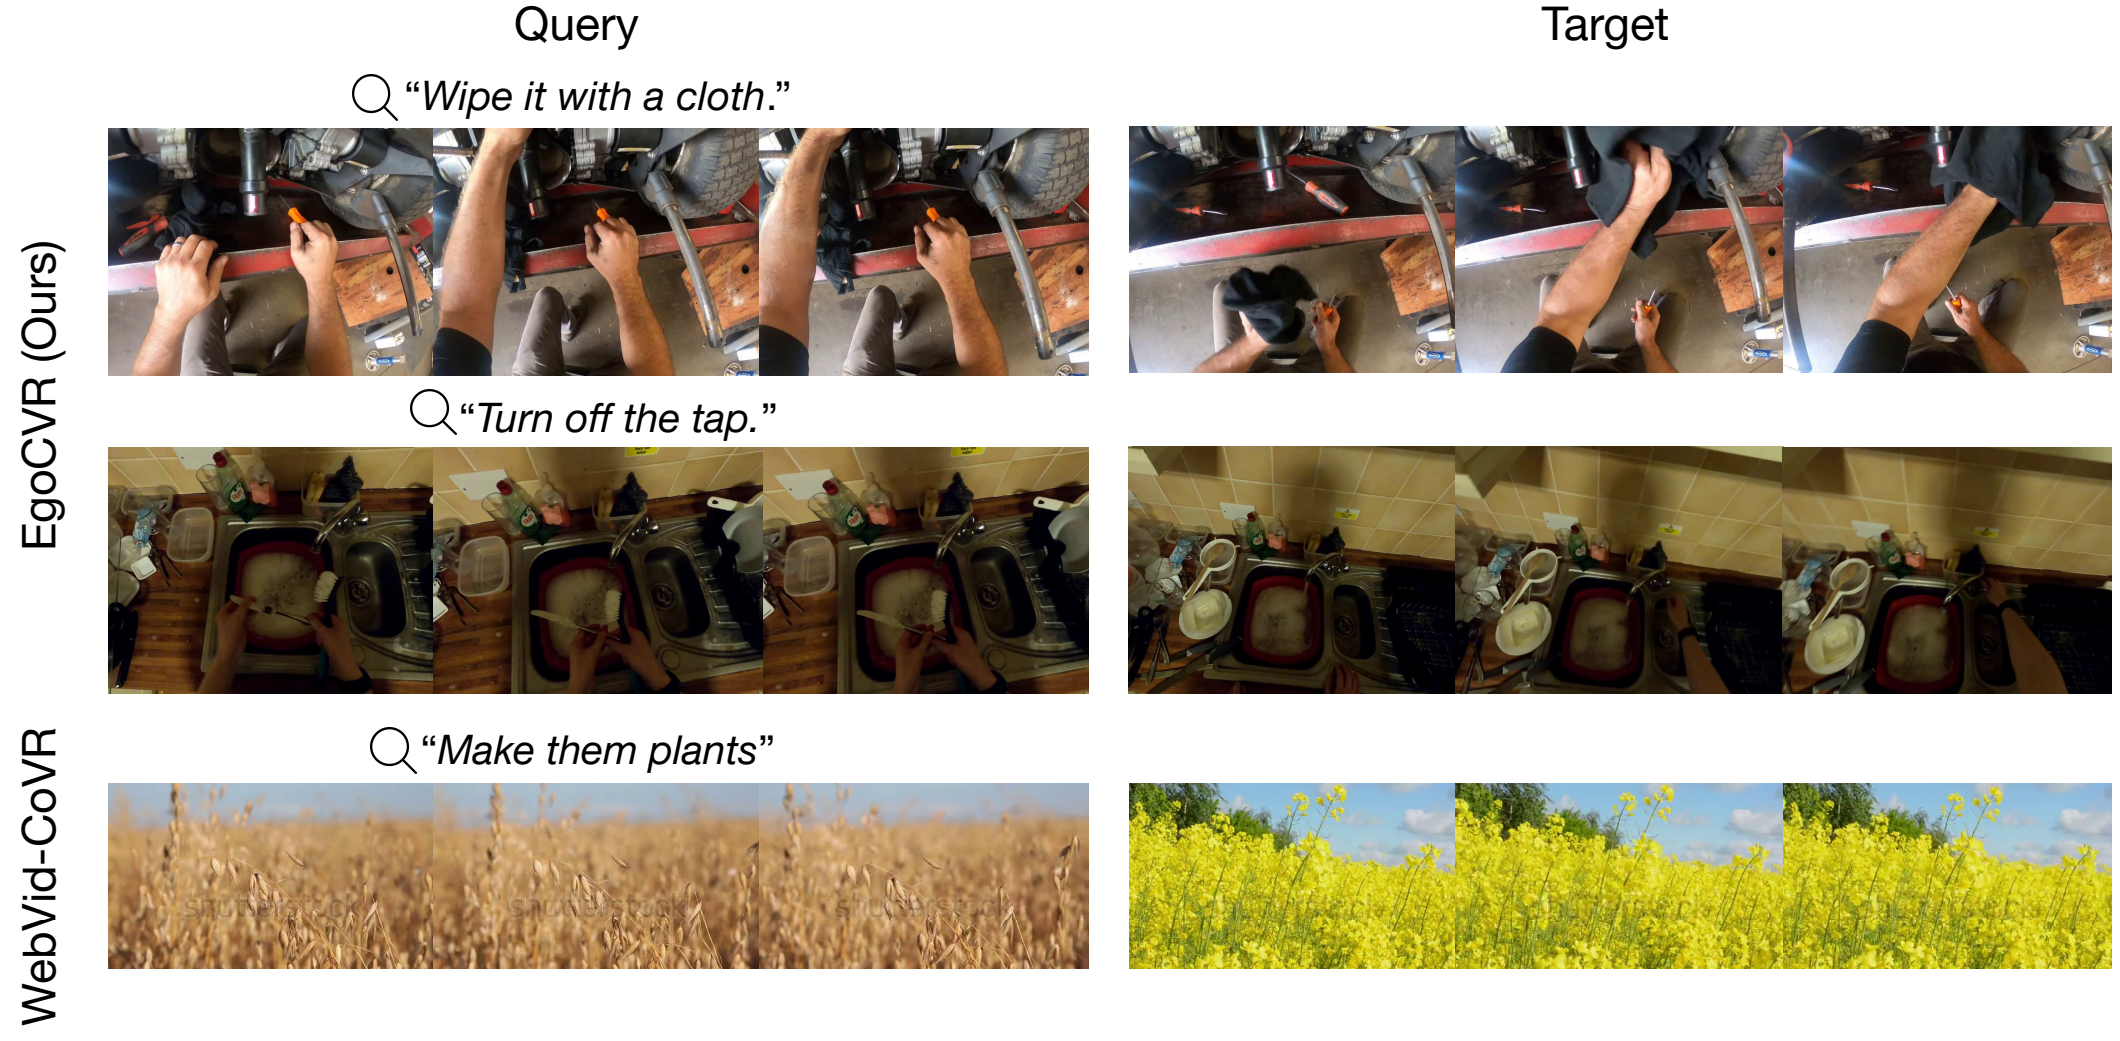
\includegraphics[scale=0.22]{egocvr-1.png}
\end{center}

\section*{Method}

\subsection*{Evaluation Dataset}
\begin{enumerate}
    \item 155k annotated clips were extracted from 1,250 long videos in the Ego4D dataset.
    \item The clips were filtered for temporal overlap, resulting in 9k distinct video clips.
    \item Pairs were manually identified from video clips in the same video, looking for similarity in captions, specifically a single action or object change, with an emphasis on temporal modifications, resulting in 2,295 high-quality pairs.
    \item GPT-4 was few-shot prompted to generate the modification text between the video pair.
    \item The authors include similar video clips that were from the same long video and don't have the same action as the target as a distraction.
\end{enumerate}

\subsection*{TFR-CVR}
\begin{enumerate}
    \item The source video is captioned and then combined with the modification text using an LLM to generate a target video caption.
    \item The target video caption is used to perform text-based retrieval.
    \item The video database is filtered for visual similarities with the source video to ensure videos are both textually relevant and visually similar.
\end{enumerate}

\begin{center}
    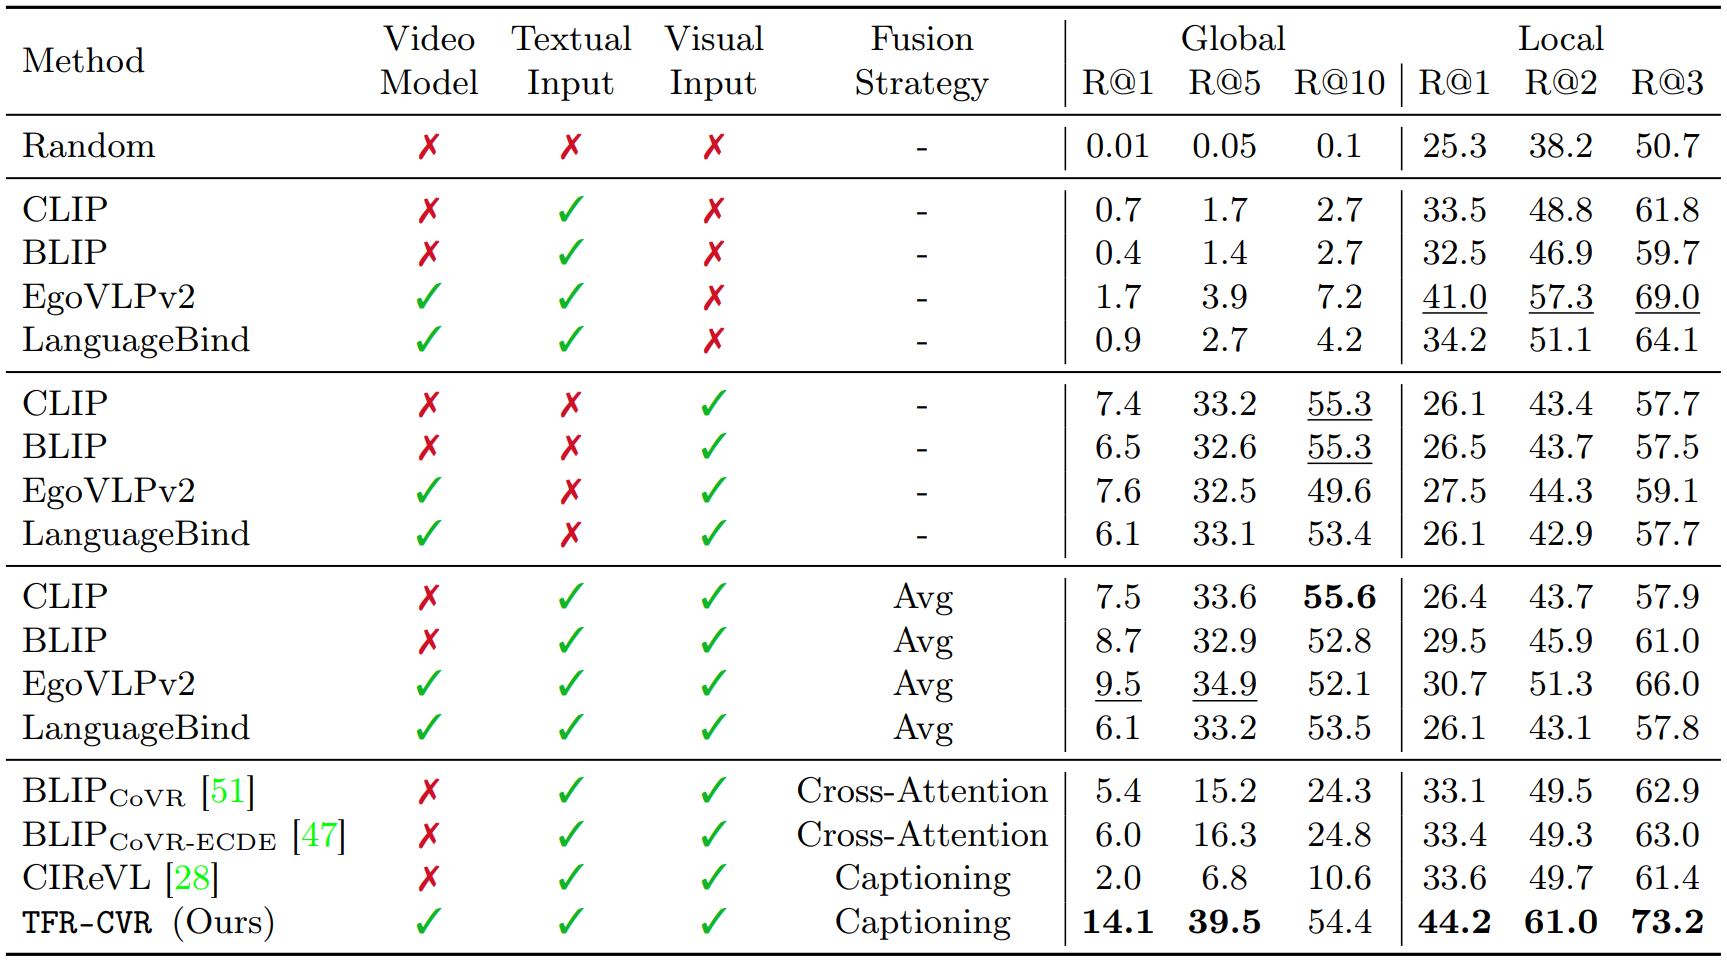
\includegraphics[scale=0.22]{egocvr-2.png}
\end{center}

\section*{Limitations}
\begin{enumerate}
    \item The benchmark does not include a training set.
    \item The dataset only consists of egocentric videos and may not generalize well to third-person videos.
    \item LLM-generated captions occasionally misrepresented the video content.
\end{enumerate}

\begin{center}
    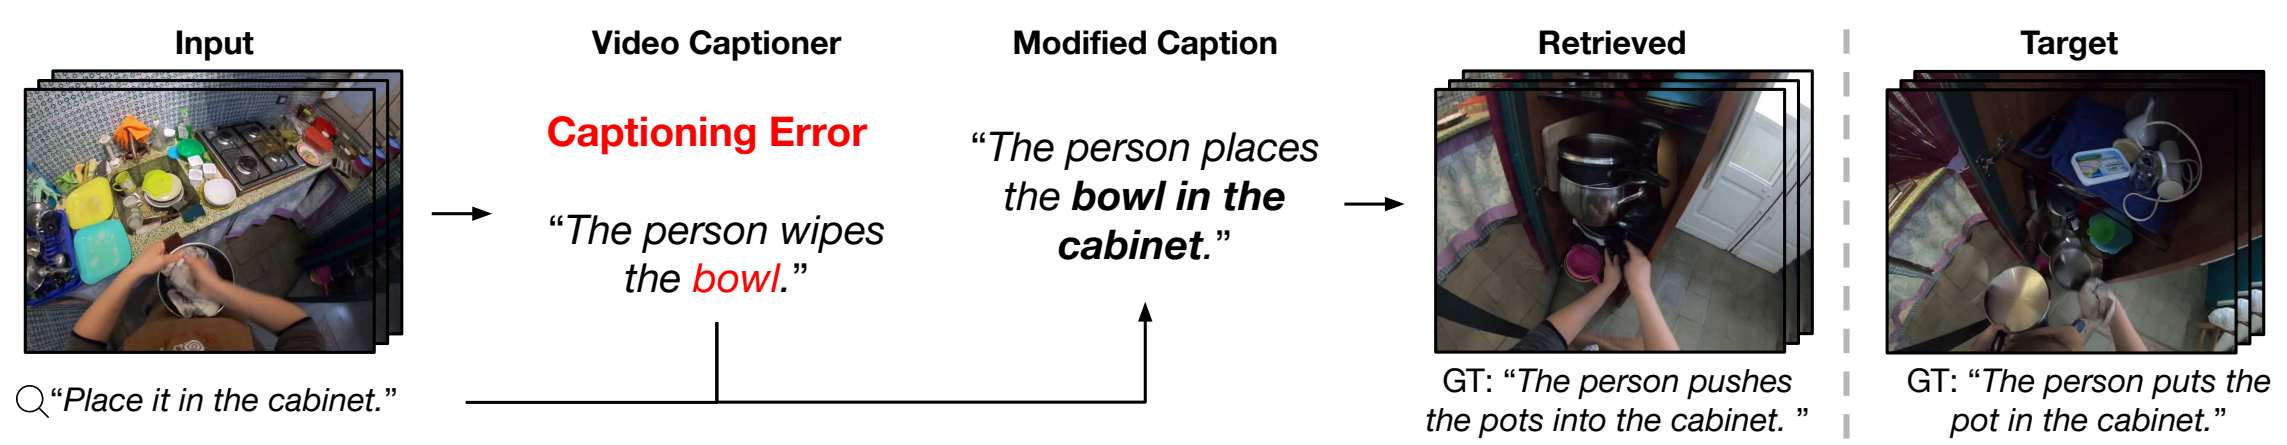
\includegraphics[scale=0.22]{egocvr-3.png}
\end{center}

\end{document}